\newpage
\section{Conclusions and Recommendation} \label{Conclusions}
\subsection{Conclusions}\label{conclusions}

In this research we investigated how useful Ampersand is for designing registry systems by analyzing legislation and regulations.
We did this in the form of \acrshort{ar}.
The case used is the \acrshort{big}.

The Ampersand method was used to analyze part of the law and to process it via scripting (see appx.~\ref{appendixAdl}) into a prototype (see appx.~\ref{appendixPrototype}) and \acrlong{ca} ( see appx.~\ref{ConceptualAnalysis}).
During the analysis phase, observations (see appx.~\ref{appendixLoglines}) were made.
These are recorded with date and time stamp.
In addition to the analysis, there were interviews (see appx.~\ref{appendixInterviews}) with a number of people from the \acrshort{cibg} organization.
During the interviews the Ampersand approach was discussed and the \acrlong{ca} and the prototype were discussed.
The collected data from observations and interview has been input for the content analysis (see appx.~\ref{appendixContentAnalysis}).

\begin{comment}
http://www.plantuml.com/plantuml/uml

@startmindmap
!theme cerulean-outline
skinparam handwritten true
* Knowledge
** Setup
***_ Docker
** Ampersand
***_ Relation Algebra
***_ Maintain knowledge
*** Gather knowledge
****_ Internet etc
*** Documentation setup
**** Script
*****_ Includes
****_ Best practices
****_ Source references
***_ Name conventions
** Overview source
***_ Annotations
** Overview script
*** Refactoring
****_ Double Concepts, relations
**_ Authorisation
** Shared components
***_ In project
***_ Over projects
**_ PHP knowledge
**_ HTML, CSS, Latex
@endmindmap\end{comment}
In addition to the main question "\acrlong{research question}" sub-questions have been defined. 
The sub-questions contribute to answering the main question.
The parts of this question are discussed in subsection~\ref{subsection:ampersand-knowledge}.
\begin{figure}[H]
    \centering
        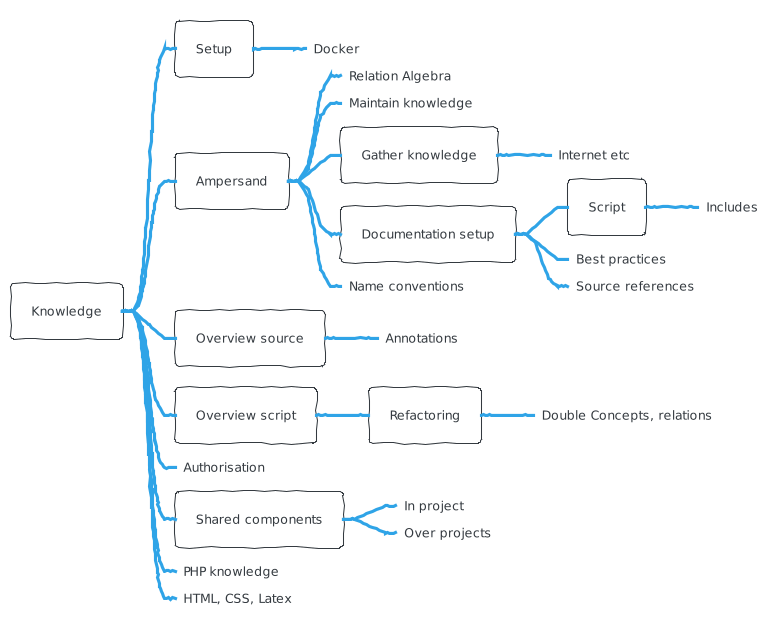
\includegraphics[width=1\textwidth]
            {knowledge.png}
        \caption{Mindmap knowledge}
    \label{fig:mindmap-knowledge}
\end{figure}

The knowledge that the software engineer needs to be able to work with Ampersand is not just limited to the knowledge of Ampersand. 
Based on the section~\ref{section:discussion} we have compiled a mindmap(see fig~\ref{fig:mindmap-knowledge} in which the matters related to the required knowledge are displayed.
The setup of Ampersand was finally set up in Docker, after we experimented with a RAP environment on the server of \acrlong{ou} and later a local environment in \acrshort{x}.
We need knowledge about the design, use and operation of Docker.
Relationship Algebra is used to create relationships between Concepts and to compose the Rules.
Knowledge of Relation Algebra in combination with Ampersand can be acquired by following the Rule-Based Design course of the \acrshort{ou}, or at least by reading the accompanying book.
When Ampersand's knowledge has been acquired, through theory and practice, it is important to keep this knowledge up to date.
Ampersand's application knowledge should be available on the Internet today, at sites like \url{https://stackoverflow.com} and other reliable information sites.
Due to a small community and, as noted earlier, low usage, the application knowledge on the internet is very limited.
To build a readable \acrlong{ca} we use the scripts of Ampersand.
For the \acrlong{ca} we use the Include statements to control build.
Best practices should be collected to simplify the start of an Ampersand project.
In these best practices things like naming (upper and lower case, CamelCase, etc) are included and proposals regarding the use of source texts.
When we are performing the analysis, there is a need for overview.
On the one hand, an overview of the treatment of the source document, ie which parts of the legal texts have already been processed and which have not yet been processed.
For this you need an annotation tool, which helps you to record the processing and helps you to keep an overview.
On the other hand, an overview is also needed during the creation of the script to be able to refactor things and avoid duplication's.
There is a tool for this, called Atlas, but it is only available in the RAP environment and not in the local setup.
Ampersand has built in a form of authorization that works over Rules and at the Interfaces.
With this authorization, a distinction can be made between user roles and the applications, in the prototype, that may be executed.
Knowledge is also required about dealing with shared Concepts.
Sharing can relate to Concepts within one project, whereby, as in the case, generic patterns with associated Concepts are shared or reused.
This form of sharing works when all components are deployed simultaneously, but it is then not possible to run different non-generic components side by side (see figure~\ref{fig:arts-deploy}, \ref{fig:tandarts-deploy} and \ref{fig:monoliet-deployment}).
The foregoing concerns sharing Concepts within a project.
Connection must be made with existing Concepts, which are not always called Concepts, within the organization.
The mapping between the Concepts found and the existing one, with which the Ampersand implementation has a relationship, must be performed.
Another form of sharing Concepts involves projects.
Defined Concepts included in Patterns will be reused by other projects.
The prototype is an HTML website in combination with CSS.
When changes are made to this, knowledge of HTML and CSS is required.
The extra functions that are not (yet) included in Ampersand can be made in PHP.
So when using this, knowledge of PHP is required.


The question regarding Concepts, Relations and Rules, which appear in the \acrshort{big}, can be referred to the appendix~\ref{ConceptualAnalysis}.
Here we find an overview of all these elements.
A finding that emerges here concerns the embedding in the software architecture of the ICT organization.
In the software architecture, the software components are managed and there is an overview of the relationships between these components.
We can see the subsystems or patterns found as software components.
It then appears that there is a certain degree of overlap of Concepts and Relations in the existing architecture and the model that Ampersand has made.
Very careful analysis is needed to discover this overlap.
The name of a Concept or Relation does not have to match, but the meaning does.
It is also possible that the naming matches, but the meaning does not.
In short, the existing software landscape needs to be carefully examined to determine which parts of the Ampersand model can be implemented
In the future, when multiple laws are analyzed to build registry systems, there may be pattern reuse.
For the legal registers, no agreements in the form of data may be shared, so no data reuse.
For example, the customer in the Donor Register may never be linked to a BIG registration with the aim of reusing customer data.

\begin{comment}
@startmindmap
!theme cerulean-outline
skinparam handwritten true
* Law
** Fitness
***_ Unambiguously 
***_ Experience
***_ Age
***_ Complexity
***_ Size
***_ completeness
** Knowledge
***_ Legal knowledge
***_ Legal reading experience
**_ Team
**_ Structure
**_ Scope
@endmindmap
\end{comment}
The question regarding the usefulness of the law for the Ampersand method has the following aspects.
\begin{figure}[H]
    \centering
        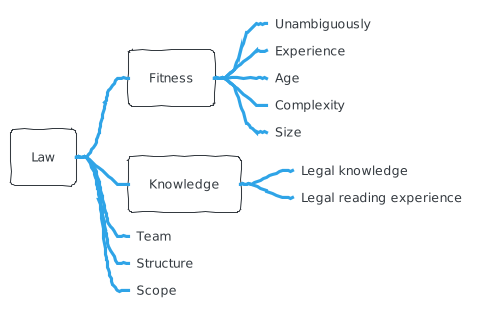
\includegraphics[width=1\textwidth]
            {law.png}
        \caption{Mindmap law}
    \label{fig:mindmap-law}
\end{figure}
We chose the \acrshort{big} to analyze it with the Ampersand method.
This law was chosen because there was a need from \acrshort{cibg} to redesign and rebuild the system that supports the law.
With Ampersand we can do the redesign.
The choice for the law was made because this law met the requirement of redesign.
During the analysis phase, we encountered a number of issues that do not support the choice and that a later choice of law should preferably comply with.
For example, the law appears to be ambiguous on some points, according to the lawyer.
Experience with the law is necessary to be able to properly analyze the law.
This is especially true if the law, such as \acrshort{big}, has options for interpretation.
The antiquity of the original law may be a cause of interpretation.
The complexity and scope of the law makes the analysis less straightforward.
When we start with the legal analysis, start with a team.
The team consists of at least one lawyer and two analysts.
This guarantees legal knowledge and experience in reading and interpreting laws and regulations.
The analysts have to keep each other on their toes when making the \acrlong{ca}.
At the start, we map out all relevant legislation and regulations and determine which legislation is included in the analysis.
After the step, the structure is determined for each part and we probably have an idea how the system can look like.
We assume here that the structure of the analysis will follow the structure of the law.
The conclusion is not that when a law is ambiguous, complex, old and large, it cannot be analyzed by Ampersand, but it does make the trajectory difficult,
One way to take is to be closer to the giver so that he is already aware when writing the law and considers the translation of the law into a registry system.
One idea is that law would already be designed directly in relation to algebra.
Then any ambiguity is gone.
This just goes to show why it is necessary to team up with a lawyer.
The lawyer can interpret the law and knows how to navigate the law.

\begin{comment}
@startmindmap
!theme cerulean-outline
skinparam handwritten true

* SWOT
** API
***_ Response
** Architecture
*** Registerkern
****_ Mapping
****_ Customization
***_ Maintenance
** Operation
***_ Process
***_ Reactive
** Tooling
***_ Atlas
***_ Excel
*** IDE
****_ Refactoring
** Deliverable
*** Conceptual analysis
****_ Testbasis
***_ Prototype
****_ Testbasis
****_ Stub
****_ CSS
** Intention of use
***_ NIH
***_ Method adoption
**_ Register systems
@endmindmap
\end{comment}
What are the strengths and weaknesses of using Ampersand for registry systems in a government organization.
\begin{figure}[H]
    \centering
        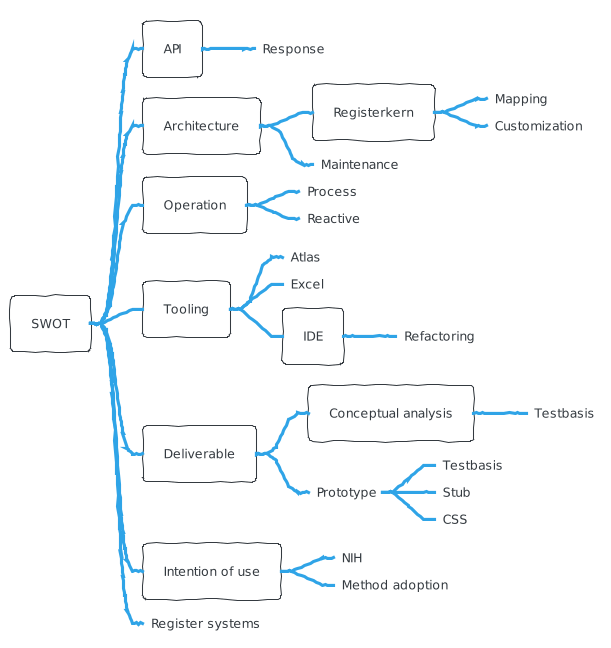
\includegraphics[width=1\textwidth]
            {swot.png}
        \caption{Mindmap swot}
    \label{fig:mindmap-swot}
\end{figure}
We can say that the analysis of a law can lead to a register system and because it is a register system, which is derived from the law, it will always be placed with a government organization.
We also concluded that there are not many observations and comments about registry systems.
Then it remains to map the strengths and weaknesses of Ampersand for a government organization and then specifically for the \acrshort{cibg}.
From the perspective of weakness and strength we will go through all parts on the basis of figure~\ref{fig:mindmap-swot}.

\parindent0em
\begin{tikzpicture}[
    pentagon/.style={%
        shape=regular polygon, regular polygon sides=5, minimum size=7.3cm, inner
        sep=-1mm, draw, fill=lightgray!75!yellow
    }, font=\scriptsize\sffamily, thick
]

% \draw[help lines] (-16,-16) grid (16,16);
\filldraw[thin,gray,fill=gray!25] (-8,-8) rectangle (8,8);
\filldraw[thin,gray,fill=white] (-7.15,-7.15) rectangle (7.15,7.15);
\draw[thin,gray] (7.15,7.15)--(8,8) (-7.15,7.15)--(-8,8) (-7.15,-7.15)--(-8,-8)
(7.15,-7.15)--(8,-8);

% Strengths
\draw[thin,gray] (-0.025,0.025)--(-7.05,0.025)--(-0.025,7.05)--cycle;
\node[pentagon,rotate=45] at (-3.75,3.75) {
    \begin{varwidth}{\linewidth}
        \begin{itemize}[leftmargin=*,noitemsep]
            \item API availabilty
            \item Integration
            \item No technical debt
            \item Reactive approach
            \item Error free specifications
            \item \acrlong{ca}
            \item Team effort
        \end{itemize}
    \end{varwidth}
};
\draw (-2,2) node[rotate=45] {\large\textbf{Strengths}};

% Weaknesses
\draw[thin,gray] (0.025,0.025)--(7.05,0.025)--(0.025,7.05)--cycle;
\node[pentagon,rotate=-45] at (3.75,3.75) {
    \begin{varwidth}{\linewidth}
        \begin{itemize}[leftmargin=*,noitemsep]
            \item API's description
            \item Manual mapping 
            \item Datamigration
            \item Documentation 
        \end{itemize}
    \end{varwidth}
};
\draw (2,2) node[rotate=-45] {\large\textbf{Weaknesses}};

% Opportunities
\draw[thin,gray] (-0.025,-0.025)--(-7.05,-0.025)--(-0.025,-7.05)--cycle;
\node[pentagon,rotate=135] at (-3.75,-3.75) {
    \begin{varwidth}{\linewidth}
        \begin{itemize}[leftmargin=*,noitemsep]
            \item API http-code response
            \item Customization \acrshort{rk}
            \item Version gap analysis
            \item Atlas local
            \item \acrlong{ca} as testbasis
            \item Stub 
        \end{itemize}
    \end{varwidth}
};
\draw (-2,-2) node[rotate=135] {\large\textbf{Opportunities}};

% Threats
\draw[thin,gray] (0.025,-0.025)--(7.05,-0.025)--(0.025,-7.05)--cycle;
\node[pentagon,rotate=-135] at (3.75,-3.75) {
    \begin{varwidth}{\linewidth}
        \begin{itemize}[leftmargin=*,noitemsep]
            \item NIH
            \item Process orientation
            \item Redundancy script and tool
            \item IDE-refactoring
        \end{itemize}
    \end{varwidth}
};
\draw (2,-2) node[rotate=-135] {\large\textbf{Threats}};
\draw(0,-7.55) node {\Large EXTERNAL};
\draw(0,7.55) node {\Large INTERNAL};
\draw(-7.55,0) node[rotate=90] {\Large POSITIVE};
\draw(7.55,0) node[rotate=270] {\Large NEGATIVE};
\draw(-0.6,0.6) node {\Huge\textbf{S}}; 
\draw(0.6,0.6) node {\Huge\textbf{W}};
\draw(-0.6,-0.6) node {\Huge\textbf{O}};
\draw(0.6,-0.6) node {\Huge\textbf{T}};
\end{tikzpicture}
\parindent2em
API availability within Ampersand at the prototype stage and many systems use APIs to communicate with the source.
The description of the APIs are missing and can be retrieved from the log.
Pushing the description of the APIs to Swagger, for example, makes it easier to use the APIs.
Adapting response from the API to the calling system would be an improvement.

The mapping from Ampersand Concepts to \acrshort{rk} is performed so that Ampersand analysis connects to \acrshort{rk}, thereby integration takes place.
This is a manual operation and can cause errors such that incorrect mappings take place or mapping does not take place.

The \acrshort{rk} has a customization that makes it possible to place register values in the editable part.
The mapping and customization will bring Ampersand and \acrshort{rk} closer together.

The issue of maintenance on the Ampersand model has been discussed before.
A strong point here is that after every maintenance a completely new model is created and no technical is introduced.
But by always setting up a completely new system, it is now not possible to migrate the data.
Ampersand systems are not used live, so the data conversion is only needed for the prototype environment.

Ampersand is a reactive designed system.
The business rules actually define the process.
The tool generates error-free specifications to support the business process.
The \acrshort{cibg} is a strong process oriented organization.

The analyst needs an overview when managing the Concepts, Relations and Rules.
Within RAP, the Atlas tool is available for this, but it is not available for the local environment.
We worked with an excel sheet during the research, but this means that things are kept up to date twice and that is of course asking for problems.
Within the IDE, the programming languages have refactoring tools at their disposal.
We have been working with \acrshort{vsc}, here the refactoring was not present and it happened that this caused inconsistency and the compile no longer ran correctly.

The \acrlong{ca} is created as deliverable.
This is used as a design for the implementation and because it is available early in the process, it can also be used as a validation tool and to base tests on.
The prototype can also be used as a test basis and real tests can be performed on this.
In combination with the API, the prototype can act in whole or in part as a stub.

For an organisation, a new method can be experienced as threatening.
It is therefore possible that one reacts with an NIH action.
To deal with this, it is wise to conduct an extensive POC and actively inform the parties.
Assemble a team and use them as promoters.
Non-ICT professionals can also be deployed as Ampersand modellers within the team, provided they have knowledge of Relation Algebra.

Ampersand should get a little more exposure than it is now just in the scientific environment.
Then it will become more known and will be used more, making it more famous again.
Now there is a certain reticence and that has the basis in the obscurity of Ampersand.

Overall conclusion is that Ampersand is a useful product for translating the law.
The output products are very useful.
Not all laws are equally suitable and the application of Ampersand in the development process must be incorporated.
The latter still requires some mission work because it is different from what people are used to and it is very unknown.
An organization will have to focus on using this and the organization is not very change-oriented.


\subsection{Recommendation}\label{recommendation}
Now that the research has been completed and the results and conclusions have been described, it is worth considering what further research could take place.
The conclusions revealed that there are omissions in the area of maintaining an overview.
In future research, attention could be given to the way in which this overview can be maintained.
This may move in the direction of annotation tools.
The follow-up research could focus on selecting and implementing tools within Ampersand for the purpose of maintaining overview.
An overview is also needed on the Concepts management side.
This seems to be possible by porting Atlas from RAP to the local environment.

Another conclusion that has been drawn is that the \acrshort{big} is not the most suitable law to analyze it via the Ampersand method.
This is not Ampersand's fault, but the law.
It is interesting to map out which requirements the law must meet in order to fit in well with the method and the follow-up is to examine how we can shape future laws that people would like to be supported by (register) systems so that they can be quickly analyzed by Ampersand.
Early participation in the legislative process could save a lot of time and money.
How much that could be, is of course fodder for a research project.

One of the interviewees feared that the Ampersand approach would take more time in the design phase than the regular approach.
The regular approach includes a more or less agile approach, in which the design is made in outline.
After which the system is cut into pieces and these are created agile.
One could research the design of two comparable systems or possibly even the same system, with one done the Ampersand way and the other the regular way.
It is then interesting to see which is faster, more complete and more workable for the follow-up process.

Another comment made during the interviews relates to the size of the system.
The hypothesis was that the system size of an Ampersand project will be smaller than the size of a system from a regular trajectory.
This could be related to the fact that Ampersand is directly on the source and does not want to include all kinds of peripheral matters.

In the context of maintaining the overview, it has been suggested to make use of the addition of XML in the source document.
So enriching the source document with the annotation XML.
The big advantage of this would be that it is then possible to generate the Ampersand script.
Especially after changes in the source document, where the existing annotations can be inserted in the new version.
This adjustment would be even more beneficial once there is an existing national base of Concepts and Relations.
The link between annotations and the national base could result in an enormous acceleration in development.
This is worth investigating, but will have to be split into several studies.

During the research we were regularly confronted with the \acrshort{rk}.
It is worth investigating how exactly this link should be established.
Where are the similarities and where are the differences?
In this context we again come across the issue of the common Concepts.
